%\subsection{Phase Two Data Analysis}
%
%\subsubsection{Comparison of Developed Abaqus Model with Literature}


In verifying the results of the model produced in Abaqus experimental data taken on the Claiborn Pell Bridge that were published in the Journal of the
Structural Division.
Upon completion in 1969 a study involving seven seismometers estimated the first 20 modes, 11 normal modal response shapes, and 20
critical damping locations.
Traffic, wind, and other environmental factors loading was measured by seismometers. The direct power spectral density by
way of the Ambient Vibrations Survey method was found of each recorded motion, estimates of the natural frequencies were produced.
An Ambient Vibration Survey (ASV) was performed on the bridge on August 20-22, 1969.
During experimentation, approximately 8,000 vehicles passed over the bridge each day
and winds were moderate. Seven seismometers were arranges in five different orientations to properly capture the modal shapes.
20 natural frequencies, 11 normal mode shapes, and 20 critical damping estimates are presented.
The First 20 modes of vibration ranged from 0.155-0.993 Hz,
modal shapes for the first 5 symmetric vertical modes can be seen in \ref{fig:Paul_Modes1-5}\\

%\begin{figure}[h]
%\centering
%\includegraphics[width=\linewidth]{Paul_Modes1-5}
%\caption{The modal response for the first five modes of the Claiborn Pell Bridge.}
%\label{fig:Paul_Modes1-5}
%\end{figure}

In table \ref{tab:FirstFive} the first five modal frequencies produced by the Abaqus model and that indicated by the Journal article. 
The fatigue that has occurred to the bridge since 1969 will account for some of the discrepancies between the frequencies as the bridge will now vibrate differently 
The maximum relative difference is \textbf{\textit{PLACEHOLDER}}, which shows that the frequencies calculated by Abaqus compare well with the measured and analyzed values. 
The main dynamic response properties of the Claiborn Pell Bridge are included in the FEM, which concur with the journal article. 
It is efficient to study the modal properties of the bridge using the FEM.


\begin{table}
\begin{tabular}{|l|l|l|l|}
\hline
Mode &  Journal Article Frequencies [Hz] & Abaqus Model Frequencies [Hz]  & Percent Difference   \\
\hline
1    & 0.16                          & 0.135                              & 15.62\%                \\
2    & 0.42                          & 0.151                           	  & 64.04\%                \\
3    & 0.52                          & 0.161                              & 69.03\%              \\
4    & 0.64                          & 0.224                              & 65.00\%            \\
5    & 0.71                          & 0.259                              & 62.51\%          \\
\hline
\end{tabular}
\caption{First five modes comparison for Abaqus and Journal Article}
\label{tab:FirstFive}
\end{table}

As the frequencies are comparable, modal shape concurrence can be looked at. The following is the modal response of the bridge as indicated by Abaqus in \ref{fig:ABAQUS_Chris}. 

\begin{figure}[h]
\centering
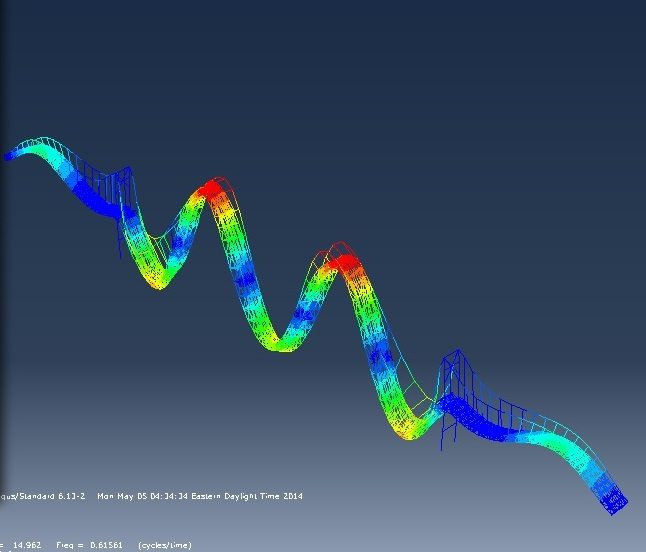
\includegraphics[scale=1]{5th_symm_vert_no_weight}
\caption{Modal Response of Abaqus Model}
\label{fig:ABAQUS_Chris}
\end{figure}
